\documentclass[12pt,a4paper]{article}
\def\ntitle{How does carbon dioxide affect human's life?} 

\usepackage{fancyhdr}
\usepackage{lastpage}
\usepackage{amsthm}
% \usepackage[sorting=none]{biblatex}
\usepackage{hyperref}
\usepackage{amsmath}
\usepackage{amsfonts}
\usepackage{siunitx}
\usepackage{mathabx}
\usepackage[inkscapelatex=false]{svg}
\usepackage{footnote}
\usepackage{tablefootnote}
\usepackage{makecell}
\usepackage[letterpaper, left=2cm,right=2cm,top=3cm,bottom=2cm]{geometry}
\usepackage{longtable}
\usepackage{multirow}
\usepackage{array}
\usepackage{verbatim}
\usepackage{minted}
\usepackage{booktabs}
\usepackage{algorithm}
\usepackage{algpseudocode}
\usepackage{subcaption}
\usepackage{graphicx}
\usepackage{subfigure}
\usepackage[toc,page]{appendix}
\usepackage[version=4]{mhchem}
\usepackage{setspace}
\usepackage{placeins}
\usepackage{wrapfig}
\usepackage{csquotes}
\usepackage[style=authoryear-ibid,backend=biber]{biblatex}
\addbibresource{EPQ.bib}

% layout
\pagestyle{fancy}
\fancyhf{}
\rhead{Page \thepage\ of \pageref*{LastPage}}
\fancyfoot[C]{\thepage}
\setlength{\headheight}{14.5pt}
\setlength{\parindent}{0pt}
\setlength{\parindent}{0em}

% title
\author{Chenyu Shi}
\date{}
\title{\Huge{\bf{\ntitle}}}

% Others

\hypersetup{
  colorlinks=true,
  urlcolor=blue,
  linkcolor=red,
  citecolor=black
}

%%%%%%%%%%%%%%%%%%%%%%%%%%
%%%%%%%%%% math %%%%%%%%%%
%%%%%%%%%%%%%%%%%%%%%%%%%%

% Theorems
\theoremstyle{definition}
\newtheorem{thm}{Theorem}[section]
\newtheorem{axiom}[thm]{Axiom}
\newtheorem{conjecture}[thm]{Conjecture}
\newtheorem{cor}[thm]{Corollary}
\newtheorem{defi}[thm]{Definition}
\newtheorem{eg}[thm]{Example}
\newtheorem{lemma}[thm]{Lemma}
\newtheorem{notation}[thm]{Notation}
\newtheorem{prop}[thm]{Proposition}

\newtheorem{question}{Question}

\newtheorem*{aim}{Aim}
\newtheorem*{assumption}{Assumption}
\newtheorem*{claim}{Claim}
\newtheorem*{ex}{Exercise}
\newtheorem*{fact}{Fact}
\newtheorem*{law}{Law}
\newtheorem*{remark}{Remark}
\newtheorem*{rrule}{Rule}
\newtheorem*{warning}{Warning}



\newenvironment{solution}{\begin{proof}[Solution]}{\end{proof}}

% Special sets
\newcommand{\C}{\mathbf{C}}
\newcommand{\R}{\mathbf{R}}
\newcommand{\Q}{\mathbf{Q}}
\newcommand{\Z}{\mathbf{Z}}
\newcommand{\N}{\mathbf{N}}
\newcommand{\F}{\mathbf{F}}
\setlength{\parindent}{0em}
% Symbols
\newcommand{\abs}[1]{\left\lvert #1\right\rvert}
\newcommand{\floor}[1]{\left\lfloor #1\right\rfloor}
\newcommand{\ceil}[1]{\left\lceil #1\right\rceil}
\newcommand{\set}[1]{\{#1\}}
\newcommand{\limit}[2]{\lim\limits_{#1\to #2}}
\renewcommand{\d}{\mathop{}\!\mathrm{d}} 
\renewcommand{\vec}[1]{\boldsymbol{\mathbf{#1}}}
\renewcommand{\P}{\mathrm{P}}
\DeclareMathOperator{\lcm}{lcm}
\DeclareMathOperator{\E}{E}
\DeclareMathOperator{\Var}{Var}

\begin{document}
    \maketitle
    \newpage
    \tableofcontents    
    \newpage
    \setlength{\parskip}{1em}   
    \setstretch{2}
    
    \section{Abstract}
    Nothing yet.
    \section{Introduction}
    As is well-known to all of us, carbon dioxide (aka. $\ce{CO2}$ in the following) accounts for roughly \label{data} of the air, and $75\%$ of the emission in the air we breathe \label{cite}. While there are a number of benefits $\ce{CO2}$ brings to human, such as helping plants to grow as necessity for photosynthesis, it actually does relatively more harm, including contributing to global warming, extreme weather conditions, ocean acidification, sea levels rise and, consequently, disruptions to ecosystems, far outweighing the benefits it brings.

    For the time being, as the advancement of technology and the improvement of human's way of life and standard of living, particularly the increasing number of automobiles on the road and growing industrial demand, the emission of $\ce{CO2}$ has significantly increased year by year, 
    $\ce{CO2}$ problem is becoming increasingly serious and urgent. Hence, in this dissertation, I will introduce, generally in the literature review, the status quo and impact of $\ce{CO2}$, and people's strategies for coping with this phenomenon; and then, concentrate on the prediction of $\ce{CO2}$ emissions and the relationship between $\ce{CO2}$ and global warming, by estabilishing several mathematical models based on data I've found.
        
    \section{Literature Review}
    \subsection{Introduction}
    In this section, I will provide an overview of the project by referencing previous studies, in order to give a general introduction to $\ce{CO2}$'s effect. Firstly, I will introduce the current $\ce{CO2}$ emission condition by analyzing ppm value and other factors while providing specific annual data. Secondly, I will focus on elaborating the influences of \ce{CO2} emission in many aspects such as ecosystem and mankind. Last, I will introduce human's response to  $\ce{CO2}$ emission, including actions of organizations and nations.
    
    \subsection{Emission Condition}
    
    Before Industrial Revolution, the concentration of $\ce{CO2}$ in atmosphere was approximately $280$ parts per million (abbr. ppm in the following) \citep{neftel_evidence_1985}. The value exploded to $377.7$ ppm in 2004, a striking rise of roughly $35\%$ \citep{dr_pieter_tans_trends_2022}. More surprisingly, according to researchers from National Oceanographic and Atmospheric Administration and Scripps Institution of Oceanography, the monthly mean $\ce{CO2}$ concentration level peaked at $421$ ppm in May 2022, which reflected an increasingly serious condition at present \citep{national_oceanographic_and_atmospheric_administration_carbon_2022}. Additionally, an Organisation for Economic Co-Operations and Development report predicts a $\ce{CO2}$ level of $685$ ppm by 2050, indicating that the prospect of dealing with $\ce{CO2}$ emission is not optimistic \citep{organisation_for_economic_co-operations_and_development_oecd_2012}.

    As for specific average $\ce{CO2}$ emission changed annually, measurements from Mauna Loa Observatory are listed in \hyperref[emission]{Table \ref*{emission}} and visualized in \hyperref[emission_line]{Figure \ref*{emission_line}}, in which we can observe the steady increase of the amount of $\ce{CO2}$ emission \citep{national_oceanographic_and_atmospheric_administration_gml_data_notitle_2023}.
    \begin{figure}[h]
        \centering
        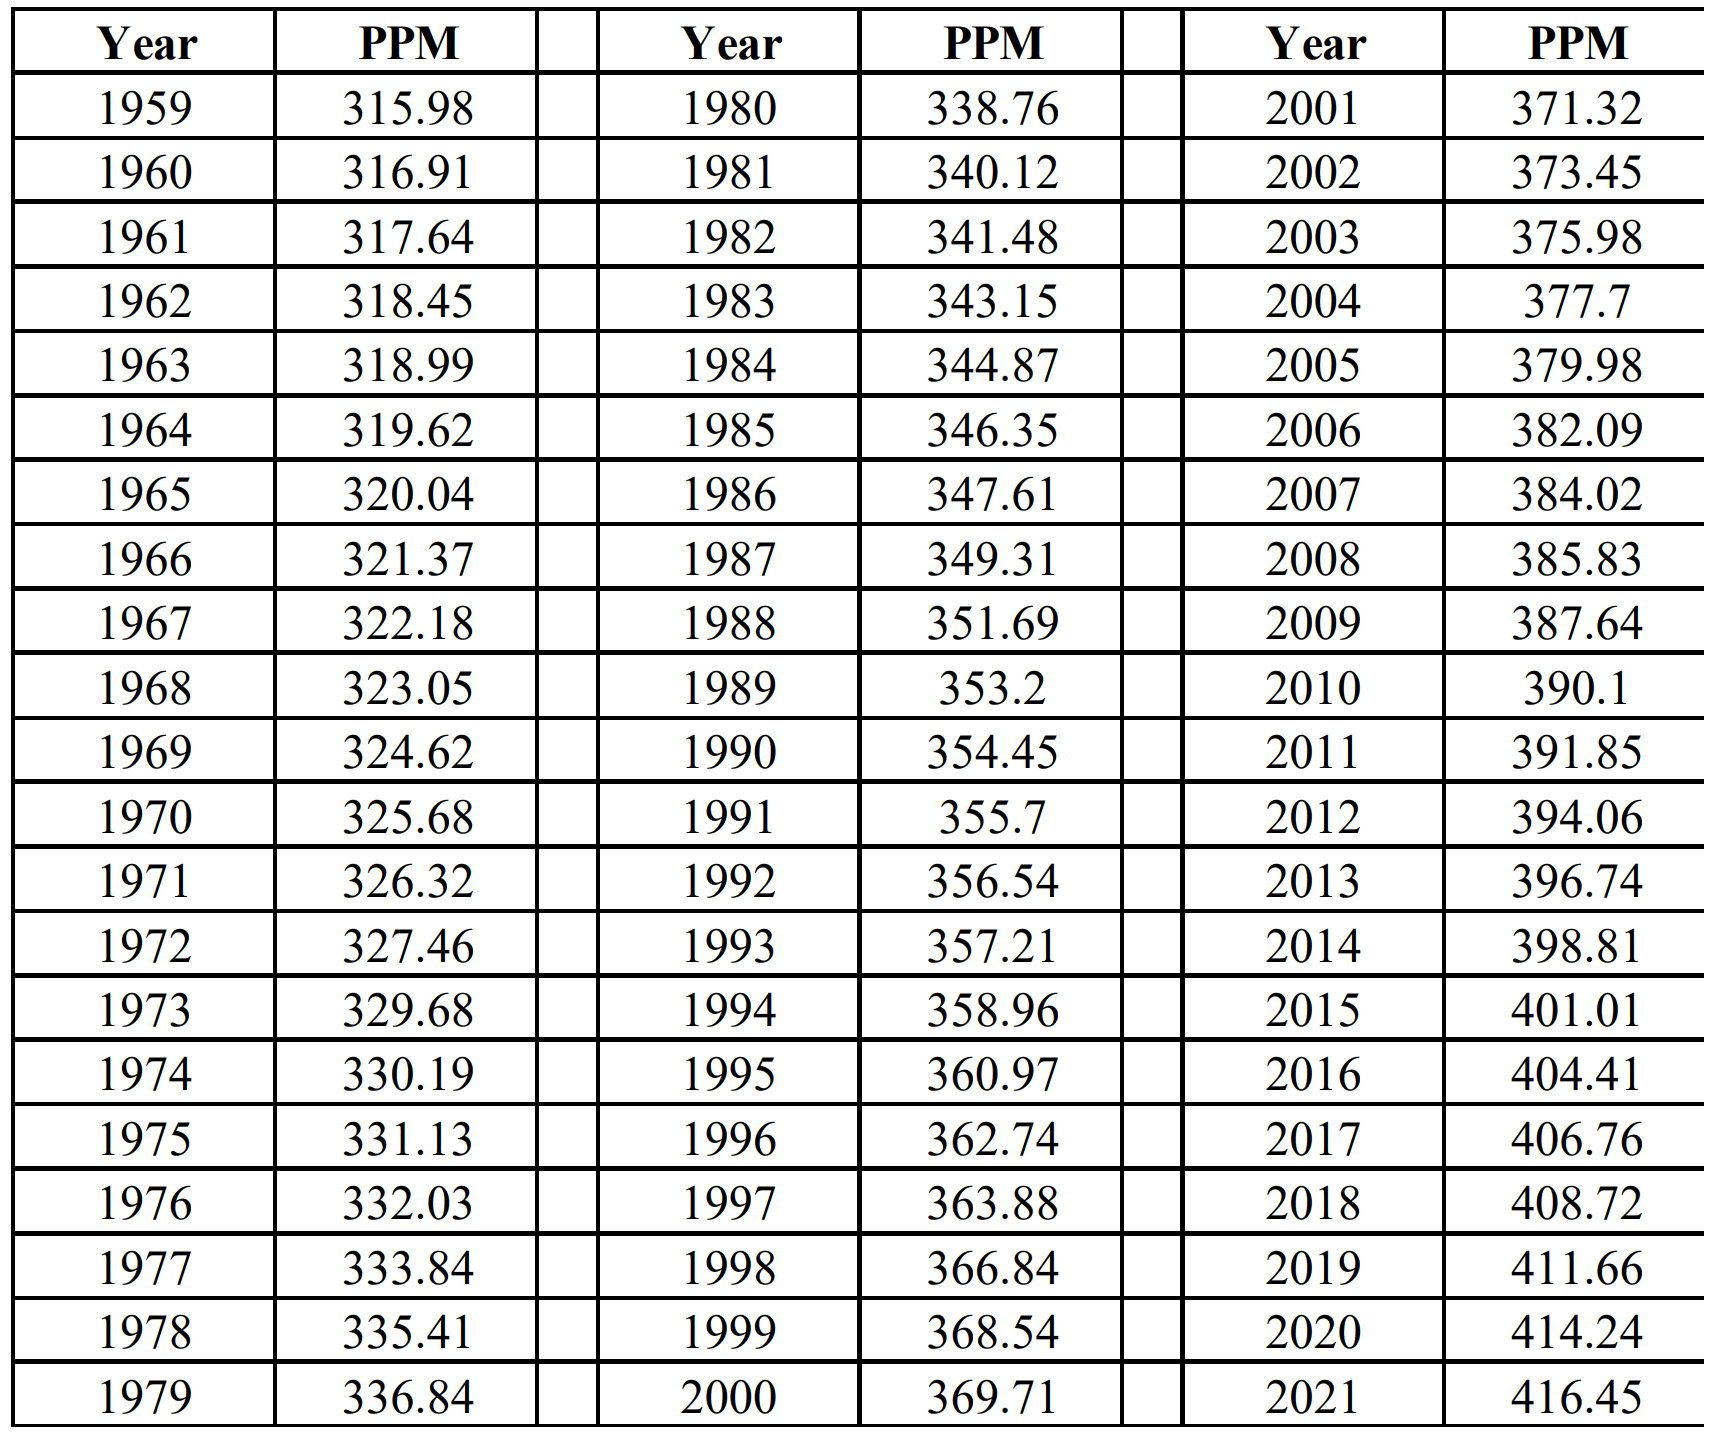
\includegraphics[width=1\linewidth]{img/emission.png}
        \captionof{table}{Average $\ce{CO2}$ emission annually}
        \label{emission}
    \end{figure}
    \begin{figure}[H]
        \centering
        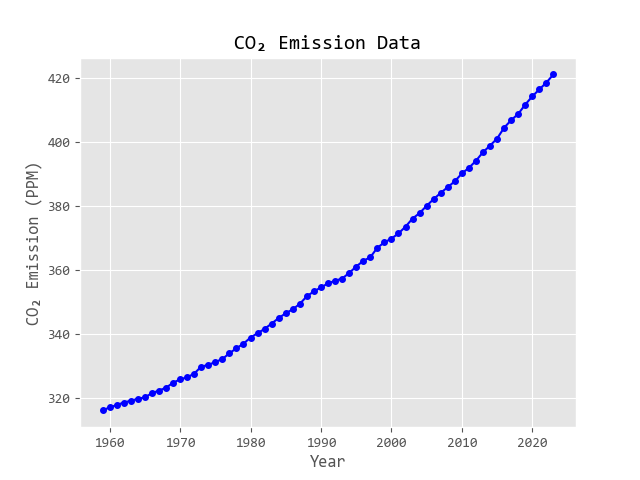
\includegraphics[width=\linewidth]{img/emission_line.png}
        \caption{$\ce{CO2}$ emission line chart}
        \label{emission_line}
    \end{figure}
    
    Apart from ppm value as elaborated above, there are other aspects discribing the emissions of $\ce{CO2}$ which is quite worth noting. As International Energy Agency reports, in 2022, the emission growth is mainly caused by extreme weather which brings about more cooling and heating demand. Despite that, it is reported that industrial emissions declined by $1.7\%$, driven by a reduction in cement and steel production in China. A good news would be the unprecedented advancement of new energy technology, including solar PV and wind energy, which reduce the $\ce{CO2}$ emissions to some extent \citep{iea_co2_2023}.
    
    \subsection{Effects}
    \subsubsection{Growth of Plants}
    As expected, $\ce{CO2}$ does play an irreplaceable role in stimulating overall biomass of plants, together with increasing the soil C:N ratio and microbial $\ce{N}$ contents \citep{de_graaff_interactions_2006}. At the same time, it is widely acknowledged and verified by many studies that the increase of atmospheric $\ce{CO2}$ concentrations also leads to the global photosynthesis rise \citep{qi-de_effects_1992}\citep{campbell_effects_1988}\citep{kramer_carbon_1981}. Other benefits of $\ce{CO2}$ include higher plant water use efficiency due to reduction in transpiration, which results in less water comsumption \citep{prior_review_2011}. Nevertheless, $\ce{CO2}$ may inhibit plant growth to some extent. For instance, higher $\ce{CO2}$ concentration may bring about reduction of concentrations of crucial nutrients such as nitrogen, phosphorus and protein \citep{conroy_influence_1992}.
    \subsubsection{Global Warming}
    As one of the greenhouse gas, $\ce{CO2}$ is widely being considered as the main driving factor that causes the phenomenon of global warming. Specifically, when the surface of earth automatically dissipate heat to the space in the form of electromagnetic waves, $\ce{CO2}$ can serve to absorb a certain wavelength range of those waves. In this way, it can help trap heat obtained from the sunlight and thus increase global temperature \citep{seim_influence_2020}. Scientists have found the positive correlation, or even a simple near-linear relation, between $\ce{CO2}$ and global temperature \citep{matthews_proportionality_2009}.

    Furthermore, global warming has led to considerable serious consequences in many different facets of life on Earth. On climates, increasing $\ce{CO2}$ concentration contributes to more precipitation at a rate of about $7\%$ per kelvin \citep{wentz_how_2007}\citep{lambert_how_2008}\citep{stephens_controls_2008}. However, what is more lethal is that by changing large-scale atmospheric circulation patterns, the growing atmospheric $\ce{CO2}$ levels may change the precipitation patterns, that is, make wet place to be wetter and dry places to be drier \citep{national_geographic_society_influence_2023}. As a result, as simulated and measured by several models, the increased frequency and intensity of heavy precipitation, along with the melting of glaciers and polar ice caps, has lead to more severe flooding, which will undoubtedly cause catastrophic consequences \citep{alifu_enhancement_2022}\citep{alfieri_global_2015}. Simultaneously, the level of drought in specific areas increased substantially and will thus bring about large threats to environment and ecosystem \citep{dai_drought_2011}\citep{zeng_increased_2023}. Apart from drought and flooding, many other extreme weather events, including hurricanes and wildfires, also occur more frequently and intensively, under the rising levels of global warming and $\ce{CO2}$ concentration \citep{anthes_hurricanes_2006}\citep{torn_predicting_1992}\citep{moore_quantifying_2015}.
    \subsubsection{Ocean Acidification}
    As we all know from the chemical knowledge that $\ce{H2O + CO2 -> H2CO3}$, when absorbing excess $\ce{CO2}$ gas, the ocean water is gradually acidified, i.e. its pH value gradually decreases. Numerous studies have revealed that the rate of acidification is progressively increasing, especially as we've entered the 21\textsuperscript{st} century \citep{doney_ocean_2009}\citep{zeebe_history_2012}. We need to recognize as well that the acidification of seawater would have devastating effects to a broad range of marine organisms \citep{guinotte_ocean_2008}. Specifically speaking, ocean acidification may lead to sensory deficits in marine organisms and have a negative impact on several physiological processes such as respiration, reproduction and excretion, which thus increases their general death rate \citep{gazeau_impacts_2013}\citep{kroeker_impacts_2013}\citep{radford_ocean_2021}. For instance, coral reefs are highly susceptible to ocean acidification due to their predominant composition of $\ce{CaCO3}$ which is likely to dissolve in acidic water, and the consequently increasing dissolution rate and reducing calcification rate pose a significant threat to the growth of coral reefs \citep{kleypas_coral_2009}\citep{silverman_coral_2009}. 
    \subsubsection{Ecosystem}
    Generally speaking, the elevated concentration of $\ce{CO2}$ inflicts substantial harm on the Earth's ecosystem. As analyzed above, the rapid increase of $\ce{CO2}$ concentration with cause dramatic change of global climate and environment, which will have a wide impact on the distribution and behavior of plant and animal species, many of wh ich may suffer a rise in mortality. Thereinto, changes in the number of key species can have cascading effects throughout food webs \citep{schindler_influence_1997}. That means, some species may be affected indirectly due to the change of their predators or food source, which can bring about an imbalance in ecosystem. At the same time, the survival of a number of species, particularly those that are less resilient to rapid environmental change, are greatly threatened under change of $\ce{CO2}$ concentration, implying shifts in the composition and structure of ecosystem and loss of biodiversity \citep{korner_biodiversity_1995}.
    \subsubsection{Mankind}
    In addition to environmental influence, the impact of elevated $\ce{CO2}$ concentration on human beings is also noteworthy. In agricultural aspect, while it is true that extreme weathers like drought may contribute to a decline in crop yield \citep{sun_does_2023}, it is found that the promoting effect of $\ce{CO2}$ to plant growth outweighs its harm, that is to say, in general, the crop yield is positively correlated to the concentration of $\ce{CO2}$ within a certain range \citep{yang_rice_2024}.

    Regarding human health, firstly, it has been found that the growing $\ce{CO2}$ concentration can have adverse effects on the nutrient content in food, specifically a decline of $5-15\%$ in protein and mineral concentrations and even up to $30\%$ in B vitamins \citep{loladze_hidden_2014}\citep{myers_increasing_2014}\citep{zhu_carbon_2018}. On top of that, research indicates that elevations in ambient $\ce{CO2}$ would pose direct risks for human health, resulting in potential health problems including inflammation, bone demineralization and endothelial dysfunction among others \citep{jacobson_direct_2019}.
    
    \subsection{Human's response}
    Confronted with such pressing issue, many organizations have made great efforts to inhibit the increase of $\ce{CO2}$ concentration. For example, in Katowice Climate Change Conference, 15 international organizations, including United Nations Framework Convention on Climate Change (UNFCCC), have made their announcements of reducing carbon emmissions to make climate neutral by actions of installing solar photovoltaic systems and efficient cooling systems, reducing air travel and so on \citep{unfccc_15_2018}. Nations are taking actions as well. Take China as an example, it has made targets to reach peak carbon emissions by 2030 and achieve carbon neutrality by 2060 \citep{xinhua_responding_2021}.
    
    \subsection{Conclusion}
    To conclude, currently, $\ce{CO2}$ emissions have increased significantly compared with pre-industrial times and are steadily rising annually. While elevated levels of $\ce{CO2}$ can promote plant growth, it may also bring about catastrophes such as global warming and ocean acidification. As a result, the global climates are disrupted and extreme weather events are more frequent. It may then threaten the survival of animals and plants, thereby jeopardizing biodiversity and harming sustainability. As for human, though rising $\ce{CO2}$ concentration helps with the algriculture development to some extent, unfortunately, studies reveal that it may pose considerable potential health problems for human beings. Therefore, organizations and nations have made plans to reduce carbon emission, and people are pulling together to address the problem by means like developing renewable energy sources.

    
    \newpage
    \section{References}
    \bibliographystyle{agsm}
    \bibliography{EPQ}
    % \printbibliography[heading=none]
    
\end{document}